\section{Drawmaha: the exact game, and the three numbers that shape everything}\label{sec:drawmaha}

\mkey{the game spec}Solver guarantees are about one exact ruleset, so the target game must be pinned before any algorithm talk --- Drawmaha has house variants (draw timing, betting rounds, declare rules), and several design choices later in this survey silently depend on which one is meant. This project's spec:

\begin{itemize}
\item \textbf{Heads-up}, blinds, \textbf{pot-limit}; version-1 action menu \{fold, check/call, pot\}, with the bet-size menu a config so multi-size solves are a re-solve, not a rewrite.
\item Each player is dealt \textbf{five hole cards}. Betting; a three-card \textbf{flop}; betting; \textbf{one draw} (discard 0--5, replace); a \textbf{turn} and betting; a \textbf{river} and betting; showdown. Four betting rounds total, one draw round (Figure~\ref{fig:streets}).
\item \textbf{Split pot, cards speak}: half to the best five-card poker hand formed by the hole cards themselves (the \emph{inner hand}), half to the best Omaha-style hand using exactly two hole cards plus three board cards (the \emph{outer hand}). One player can \emph{scoop} both halves.
\item \textbf{Draw-count is public; identities are hidden.} Both players see how many cards each drew, never which. House rule adopted: \textbf{drawing exactly one} exposes the replacement face up, and the drawer may keep it or reject it for a face-down second card --- an extra public signal and an extra decision node unique to this project.
\end{itemize}

\begin{fullbleed}
\begin{figure}[t]
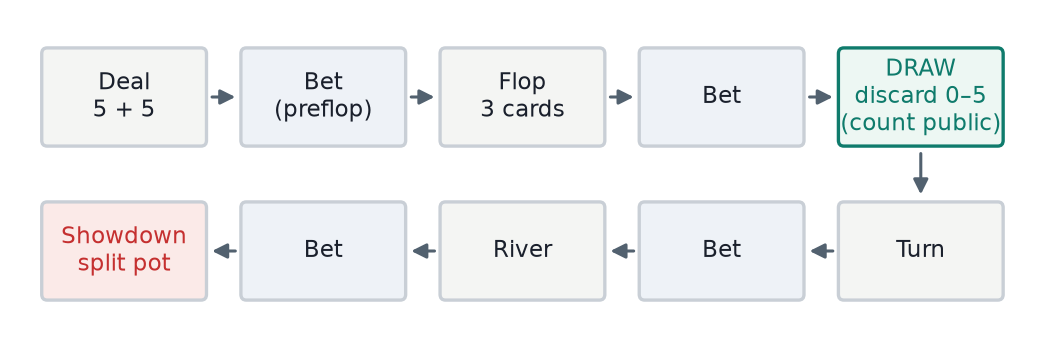
\includegraphics[width=6.45in]{figures/streets.png}
\caption{The street structure of the target game: four betting rounds, one draw round, split-pot showdown.}
\label{fig:streets}
\end{figure}
\end{fullbleed}

\subsection*{Why this game is hard: three separate blow-ups}

\mkey{three blow-ups}Comparing against the games the literature has already conquered isolates exactly what is new. Drawmaha combines three complications that existing work has faced only one at a time:

\begin{center}
\footnotesize
\begin{tabular}{@{}llll@{}}
\toprule
 & Hold'em & Pot-limit Omaha & \textbf{Drawmaha} \\
\midrule
Starting hands & 1{,}326 & 270{,}725 & \textbf{2{,}598{,}960} \\
\quad after suit isomorphism & 169 & $\sim$16{,}500 & \textbf{134{,}459} \\
Draw rounds & 0 & 0 & \textbf{1} (32 discard subsets) \\
Pot & single & single & \textbf{split} (inner + outer) \\
Betting rounds & 4 & 4 & 4 \\
\bottomrule
\end{tabular}
\end{center}

\textbf{Blow-up 1: the hand space.} $\binom{52}{5} = 2{,}598{,}960$ private hands per player --- roughly $2{,}000\times$ hold'em. Dealing both players runs to $\binom{52}{5}\binom{47}{5} \approx 4.0\times10^{12}$ deals before the board or draws multiply it. Every table, buffer, range vector, and dashboard grid in this survey has to survive this number; it is why the project's endgame is a network rather than a table (Section~\ref{sec:deepcfr}), and why a raw DeepStack-style range input does not port (Section~\ref{sec:search}). The one free win is \keyterm{suit isomorphism}\mdef{suit isomorphism}{hands identical up to relabeling suits play identically; merging them is provably lossless}: relabeling suits collapses the 2.6M hands to \textbf{134{,}459} canonical classes --- a $19.3\times$ reduction that costs nothing (Section~\ref{sec:abstraction}).

\textbf{Blow-up 2: the draw round.} The draw inserts a player-\emph{chosen} chance event mid-hand: choosing which of $2^5=32$ subsets to keep is an action; the replacement cards are chance. Its strategic signature is that \hlight{the draw count is public information --- standing pat announces strength (or a bluff, the classic ``snow''), and drawing three announces weakness --- so both players' full draw-count histories belong in the infoset.} The closest solved precedents (2-7 triple draw, badugi) are commercial, not academic; their one loud lesson is that discard \emph{identity} (which cards you threw) drives blocker effects worth real EV (Section~\ref{sec:precedents}).

\textbf{Blow-up 3: the split pot.} Cheapest of the three, and the literature says exactly why: a split pot changes only the \emph{terminal payoff function} --- who gets how much at showdown --- and never the information structure of the tree. Any CFR variant runs unmodified once the leaves pay out correctly; the engineering moves into a fast dual evaluator (inner-hand rank and outer-hand rank per showdown) and into strategy itself becoming two-dimensional: a hand now has inner equity, outer equity, and a scoop probability, which haunts abstraction (Section~\ref{sec:abstraction}) and evaluation units (Section~\ref{sec:evaluation}).

\mnote{Searched: Semantic Scholar, arXiv, GitHub, commercial solver market, poker forums. Nothing for ``Drawmaha'' or ``Sviten Special.''}One more fact frames the whole project: the literature sweep behind this survey searched academic and commercial channels for any Drawmaha solver, bot, or analysis and found \textbf{nothing} --- the game is documented (rules sites, online mixed games) but unstudied. The ``first Drawmaha solver'' claim stands as of August 2026, with a consequence for evaluation: there is no external baseline to beat, so the project must manufacture its own opponents (Section~\ref{sec:evaluation}).
